\documentclass[handout]{beamer}
%\beamertemplateshadingbackground{brown!70}{yellow!10}
\mode<presentation>
{
  %\usetheme{Warsaw}
  \usecolortheme{crane}
  % or ...

%  \setbeamercovered{transparent}
  % or whatever (possibly just delete it)
}
\setbeamertemplate{navigation symbols}{}
\setbeamertemplate{footline}[frame number]{}
\usepackage{tikz,pgfplots}
\pgfplotsset{compat=newest}
\usepackage[utf8]{inputenc}
\usetikzlibrary{patterns}
\usepackage{amssymb}
\usepackage{amsmath}
\usepackage{colortbl}
%\usepackage{multicol}
\usepackage{cancel}
\usepackage{ulem}
\usepackage{multirow}
\usepackage{relsize}
\usepackage{algorithm}
\usepackage{algorithmic}
\usepackage{forloop}% http://ctan.org/pkg/forloop
\newcounter{loopcntr}
\newcommand{\rpt}[2][1]{%
  \forloop{loopcntr}{0}{\value{loopcntr}<#1}{#2}%
}
%\pagestyle{plain}
%\input{defs2}
\def\opt{{\textsc{OPT}_k}}
\def\const{{\mathrm{const}}}
\def\nnz{{\mathrm{nnz}}}
\def\r{\sfrac{\sigma_{\w}^2}{\sigma_{\xib}^2}}
\def\rm{\sfrac{\sigma_{\xib}^2}{\sigma_{\w}^2}}
\def\cmark{\Green{\checkmark}}
\def\xmark{\Red{\large\sffamily x}}
\newcommand{\pdet}{{\mathrm{pdet}}}
\newcommand{\MSPE}[1] {{\mathrm{MSPE}\big[#1\big]}}
\newcommand{\MSE}[1] {{\mathrm{MSE}\big[#1\big]}}
\def\Poisson{{\operatorname{Poisson}}}
\def\PB{{\operatorname{PB}}}
\newcommand{\DP}[1]{\mathcal{DP}^{#1}}
\def\Ic{\mathcal{I}}
\def\Jc{\mathcal{J}}
\def\Mc{\mathcal M}
\def\Ec{\mathcal E}
\def\sr{{\mathrm{sr}}}
\def\ktd{{k^{\underline{d}}}}
\def\Det{{\mathrm{Det}}}
\def\detu{{\widecheck{\mathrm{Det}}_\mu^\gamma}}
\def\deto{{\widehat{\mathrm{Det}}_\mu^\gamma}}
\def\Zu{{\widecheck{Z}_\mu^{\gamma}}}
\def\Zo{{\widehat{Z}_\mu^{\gamma}}}
\def\Zun{{\widecheck{Z}_\mu^{\gamma_n}}}
\def\Zon{{\widehat{Z}_\mu^{\gamma_n}}}
\newcommand{\Er}{\mathrm{Er}}
\newif\ifDRAFT
\DRAFTtrue
\ifDRAFT
\newcommand{\marrow}{\marginpar[\hfill$\longrightarrow$]{$\longleftarrow$}}
\newcommand{\niceremark}[3]
   {\textcolor{red}{\textsc{#1 #2:} \marrow\textsf{#3}}}
\newcommand{\ken}[2][says]{\niceremark{Ken}{#1}{#2}}
\newcommand{\manfred}[2][says]{\niceremark{Manfred}{#1}{#2}}
\newcommand{\michael}[2][says]{\niceremark{Michael}{#1}{#2}}
\newcommand{\michal}[2][says]{\niceremark{Michal}{#1}{#2}}
\newcommand{\feynman}[2][says]{\niceremark{Feynman}{#1}{#2}}
%\usepackage[inline]{showlabels}
\else
\newcommand{\ken}[1]{}
\newcommand{\michael}[1]{}
\newcommand{\michal}[1]{}
\newcommand{\feynman}[1]{}
\fi
\newcommand{\norm}[1]{{\| #1 \|}}

\newcommand{\deff}{d_{\textnormal{eff}}}
\def\ee{\mathrm{e}}
\newcommand\mydots{\makebox[1em][c]{.\hfil.\hfil.}}
\def\Sd{\mathscr{S}_{\!d}}
\newcommand{\dx}{\dxy_{\!\cal X}}
\newcommand{\dxk}{\dxy_{\!\cal X}^k}
\newcommand{\dk}{\dxy^k}
\newcommand{\dxy}{\mathrm{D}}
\def\simiid{\overset{\textnormal{\fontsize{6}{6}\selectfont
i.i.d.}}{\sim}}
%\newcommand{\Dxy}{D_{\!\cal X\!,\cal Y}}
\def\vskx{{\mathrm{VS}_{\!\dx}^k}}
\def\vsk{{\mathrm{VS}_{\!D}^k}}
\def\vskxm{{\mathrm{VS}_{\!\dx}^{k-1}}}
\def\vskm{{\mathrm{VS}_{\!D}^{k-1}}}
\def\vsdx{{\mathrm{VS}_{\!\dx}^d}}
\def\vsd{{\mathrm{VS}_{\!D}^d}}
\newcommand{\vs}[1]{{\mathrm{VS}_{\!D}^{#1}}}
\newcommand{\sigd}{\boldsymbol\Sigma_{\!\dx}}
\def\wols{\w_{\mathrm{LS}}}
\def\wds{\boldsymbol\w_{\!D}^*}
\def\kd{K_{\!\dx}}

\def\poly{{\mathrm{poly}}}
\def\polylog{{\mathrm{polylog}}}
\def\DPP{{\mathrm{DPP}}}
\def\DPPcor{{\DPP_{\!\mathrm{cor}}}}
\def\DPPens{{\DPP_{\!\mathrm{ens}}}}
\newcommand{\DPPreg}[1]{{\DPP_{\!\mathrm{reg}}^{#1}}}
\def\Vol{{\mathrm{VS}}}
\def\Lev{{\mathrm{Lev}}}
\newcommand\todod[1]{\Red{\# DH: #1}}
\newcommand{\explain}[2]{\mathrel{\overset{\makebox[0pt]{\text{\tiny
#1}}}{#2}}}
\def\tot {{\mathrm{tot}}}
\def\checkmark{\tikz\fill[scale=0.4](0,.35) -- (.25,0) --
(1,.7) -- (.25,.15) -- cycle;}
\newcommand{\mnote}[1]{{\bf\large \Magenta{*}}\marginpar{\small \Magenta{#1}}}
\newcommand{\bnote}[1]{{\bf #1}}

\newcommand{\sqrtshort}[1]{{\sqrt{\white{\Big|}\!\!\smash{\text{\fontsize{9}{9}\selectfont$#1$}}}}}
\newenvironment{proofof}[2]{\par\vspace{2mm}\noindent\textbf{Proof of {#1} {#2}}\ }{\hfill\BlackBox}
\newcommand{\sets}[2]
{{\hspace{-0.3mm}[\hspace{-0.3mm}#1\hspace{-0.3mm}]\hspace{-0.3mm}\choose
\hspace{-0.3mm}#2\hspace{-0.3mm}}}
\DeclareMathOperator{\sgn}{\textnormal{sgn}}
\DeclareMathOperator{\adj}{\textnormal{adj}}
\def\Rb{{\mathbf{R}}}
\DeclareMathOperator{\ws}{\widetilde{\w}}
\newcommand{\inote}[1]{{\bf {#1}}}
\def\xib{\boldsymbol\xi}
\def\Sigmab{\mathbf{\Sigma}}
\def\Sigmabh{\widehat{\Sigmab}}
\def\Sigmabt{\widetilde{\Sigmab}}
\def\S{\mathbf{S}}
\def\T{\mathbf{T}}
\def\xt{\tilde{x}}
\def\xbt{\widetilde{\x}}
\def\xbh{\widehat{\x}}
\def\ubh{\widehat{\u}}
\def\dom {{\mathrm{dom}}}
\def\val {{\mathrm{val}}}
\def\out {{\mathrm{out}}}
\def\iin  {{\mathrm{iin}}}
\def\s {\mathbf{s}}
\def\q {\mathbf{q}}
\def\qt{\tilde{q}}
\def\itld {j}
\def\ubt {\tilde{\u}}
\def\n{\{1..n\}}
\def\cb {\mathbf{c}}
\def\cW{\mathcal W}
\def\Xt{\widetilde{X}}
\def\Dbt{\widetilde{\D}}
\def\xtb{\tilde{\mathbf{x}}}
\def\ytb{\tilde{\mathbf{y}}}
\def\Xtb{\widetilde{\mathbf{X}}}
\def\Xbb{\overline{\X}}
\def\Xb{{\bar{\X}}}
\def\ybb{\overline{\y}}
\def\f{{\mathbf{f}}}
\def\g{{\mathbf{g}}}
\def\fbb{{\overline{\f}}}
\def\fb{{\overline{f}}}
\def\Xc{\mathcal{X}}
\def\W{\mathbf W}
\def\L{\mathbf{L}}
\def\Rb{\mathbf R}
\def\Pc{\mathcal{P}}
\def\Nc{\mathcal{N}}
\def\Pt{\widetilde{P}}
\def\Hc{\mathcal{H}}
\def\Wc{\mathcal{W}}
\def\Cc{\mathcal{C}}
\def\p{\mathbf p}
%\def\r{\mathbf r}
\def\Y{\mathbf Y}
\def\H{\mathbf H}
\def\K{\mathbf K}
\def\Kh{\widehat{K}}
\def\Kbh{{\widehat{\K}}}
\def\Q{\mathbf Q}
\def\Qbar{{\bar{\mathbf Q}}}
\def\Ytb{\widetilde{\mathbf{Y}}}
\def\c{{n-d\choose s-d}}
\DeclareMathOperator{\Proj}{Proj}
\newcommand{\Span}{\mathrm{span}}
\newcommand{\ofsubt}[1]{\mbox{\scriptsize \raisebox{0.25pt}{$(#1)$}}}
%\raisebox{0.5pt}{$($}}#1\mbox{\tiny \raisebox{0.5pt}{$)$}}}
\newcommand{\ofsub}[1]{\mbox{\small \raisebox{0.0pt}{$(#1)$}}}
%\newcommand{\ofsubb}[1]{\mbox{\footnotesize \raisebox{0.5pt}{$(#1)$}}}
%\newcommand{\ofsub}[1]{(#1)}
%\newcommand{\ofsub}[1]{\mbox{\tiny$|$\hspace{-0.5pt}\raisebox{-0.5pt}{$#1$}}}
\newcommand{\of}[2]{{#1{\!\ofsub{#2}}}}
\newcommand{\oft}[2]{{#1{\!\ofsubt{#2}}}}
\newcommand{\fof}[2]{{#1({#2})}}
\newcommand{\yof}[2]{{#1{\ofsub{#2}}}}
%\newcommand{\yofb}[2]{{#1{\ofsubb{#2}}}}
\newcommand{\lazy}{FastRegVol}
\newcommand{\volsamp}{RegVol}

\newcommand{\Sm}{{S_{-i}}}
\newcommand{\Sp}{{S_{+i}}}
\ifx\BlackBox\undefined
\newcommand{\BlackBox}{\rule{1.5ex}{1.5ex}}  % end of proof
\fi
%\renewcommand{\dagger}{+}
\DeclareMathOperator*{\argmin}{\mathop{\mathrm{argmin}}}
\DeclareMathOperator*{\argmax}{\mathop{\mathrm{argmax}}}
\DeclareMathOperator*{\diag}{\mathop{\mathrm{diag}}}
\def\x{\mathbf x}
\def\y{\mathbf y}
\def\ybh{\widehat{\mathbf y}}
\def\ybb{\bar{\mathbf y}}
\def\xbb{\bar{\mathbf x}}
\def\yb{{\bar y}}
\def\ybt{\widetilde{\mathbf y}}
\def\yh{\widehat{y}}
\def\yhb{\widehat{\y}}
\def\yt{\widetilde{y}}
\def\z{\mathbf z}
\def\a{\mathbf a}
\def\b{\mathbf b}
\def\w{\mathbf w}
\def\v{\mathbf v}
\def\m{\mathbf m}
\def\wbh{\widehat{\mathbf w}}
\def\wh{\widehat{\mathbf w}}
\def\vbh{\widehat{\mathbf v}}
\def\wbt{\widetilde{\mathbf w}}
\def\e{\mathbf e}
\def\zero{\mathbf 0}
\def\one{\mathbf 1}
\def\u{\mathbf u}
\def\ubbar{\bar{\mathbf u}}
\def\f{\mathbf f}
\def\ellb{\boldsymbol\ell}

\def\X{\mathbf X}
\def\Xs{\widetilde{\X}}
\def\B{\mathbf B}
\def\A{\mathbf A}
\def\C{\mathbf C}
\def\U{\mathbf U}
\def\Ubt{\widetilde{\mathbf U}}
\def\Ubh{\widehat{\mathbf U}}
\def\Ubbar{\bar{\mathbf U}}
\def\F{\mathbf F}
\def\D{\mathbf D}
\def\V{\mathbf V}
\def\M{\mathbf M}
\def\Mh{\widehat{\mathbf M}}
%\def\S{\mathbf S}
\def\Stb{\widetilde{\mathbf{S}}}
\def\Sbh{\widehat{\mathbf{S}}}
\def\St{\widetilde{\S}}
\def\Sh{\widehat{S}}
\def\Sc{\mathcal{S}}
\def\Fc{\mathcal{F}}
\def\Vc{\mathcal{V}}
\def\Bc{\mathcal{B}}
\def\Dc{\mathcal{D}}
\def\Z{\mathbf Z}
\def\Zbh{\widehat{\mathbf Z}}
\def\Zbt{\widetilde{\mathbf Z}}
\def\Abh{\widehat{\mathbf A}}
\def\I{\mathbf I}
\def\Ic{\mathcal I}
\def\II{\mathbf {I \!\,I}}
%\def\II{\boldsymbol {\mathbb I}}
\def\A{\mathbf A}
\def\P{\mathbf P}
\def\Ph{\widehat{\mathbf P}}
\def\cP{\mathcal P}
\def\cR{\mathcal R}
\def\Xt{\widetilde{\mathbf{X}}}
\def\Xh{\widehat{\mathbf{X}}}
\def\Rh{\widehat{R}}
\def\Ot{\widetilde{O}}
\def\At{\widetilde{\A}}


\def\E{\mathbb E}
\def\R{\mathbb R}
\def\N{\mathbb N}
\def\Pr{\mathrm{Pr}}
%\def\C{\mathbb C}
\def\tr{\mathrm{tr}}
\def\Sbar{{\bar{S}}}
\def\cS{{\mathcal{S}}}
\def\Tbar{{\bar{T}}}
\def\Tt{{\widetilde{T}}}
\def\rank{\mathrm{rank}}
\def\Prob{\mathrm{Prob}}
\def\Var{\mathrm{Var}}
\def\Xinv{(\X^\top\X)^{-1}}
\def\XinvS{(\X_S\X_S^\top)^{-1}}
\def\ABinvS{(\A_S\B_S^\top)^{-1}}
\def\ABinv{(\A\B^\top)^{-1}}
\def\xinv{\x_i^\top\Xinv\x_i}
\def\Xinvr{(\lambda\I+\X_{-1}^\top\X_{-1})^{-1}}
\def\pdet{\mathrm{pdet}}
\newcommand{\vol}{\mathrm{vol}}
%\newcommand{\defeq}{:=}
\newcommand{\defeq}{\stackrel{\textit{\tiny{def}}}{=}}
\newcommand{\di}{{[d+1]_{-i}}}
\newcommand{\cov}{\mathrm{cov}}
\let\origtop\top
\renewcommand\top{{\scriptscriptstyle{\origtop}}} % this makes transpose not so big

\definecolor{silver}{cmyk}{0,0,0,0.3}
\definecolor{yellow}{cmyk}{0,0,0.9,0.0}
\definecolor{reddishyellow}{cmyk}{0,0.22,1.0,0.0}
\definecolor{black}{cmyk}{0,0,0.0,1.0}
\definecolor{darkYellow}{cmyk}{0.2,0.4,1.0,0}
\definecolor{orange}{cmyk}{0.0,0.7,0.9,0}
\definecolor{darkSilver}{cmyk}{0,0,0,0.1}
\definecolor{grey}{cmyk}{0,0,0,0.5}
\definecolor{darkgreen}{cmyk}{0.6,0,0.8,0}
\newcommand{\Red}[1]{{\color{red}  {#1}}}
\newcommand{\Purple}[1]{{\color{purple}  {#1}}}
\newcommand{\Magenta}[1]{{\color{magenta}{#1}}}
\newcommand{\Green}[1]{{\color{darkgreen}  {#1}}}
\newcommand{\Blue}[1]{\color{blue}{#1}\color{black}}
\newcommand{\Orange}[1]{\textcolor{orange}{#1}\color{black}}
\newcommand{\Brown}[1]{{\color{brown}{#1}\color{black}}}
\newcommand{\Grey}[1]{{\color{grey}{#1}\color{black}}}
\newcommand{\white}[1]{{\textcolor{white}{#1}}}
\newcommand{\yellow}[1]{{\textcolor{reddishyellow}{#1}}}
\newcommand{\darkYellow}[1]{{\textcolor{darkYellow}{#1}}}
\newcommand{\grey}[1]{{\textcolor{grey}{#1}}}

\DeclareMathOperator{\half}{\frac{1}{2}}

\ifx\proof\undefined
\newenvironment{proof}{\par\noindent{\bf Proof\ }}{\hfill\BlackBox\\[2mm]}
\fi

\ifx\theorem\undefined
\newtheorem{theorem}{Theorem}
\fi

\ifx\example\undefined
\newtheorem{example}{Example}
\fi

\ifx\condition\undefined
\newtheorem{condition}{Condition}
\fi
\ifx\property\undefined
\newtheorem{property}{Property}
\fi

\ifx\lemma\undefined
\newtheorem{lemma}{Lemma}
\fi

\ifx\proposition\undefined
\newtheorem{proposition}{Proposition}
\fi

\ifx\remark\undefined
\newtheorem{remark}{Remark}
\fi

\ifx\corollary\undefined
\newtheorem{corollary}{Corollary}
\fi

\ifx\definition\undefined
\newtheorem{definition}{Definition}
\fi

\ifx\conjecture\undefined
\newtheorem{conjecture}{Conjecture}
\fi

\ifx\axiom\undefined
\newtheorem{axiom}{Axiom}
\fi

\ifx\claim\undefined
\newtheorem{claim}{Claim}
\fi

\ifx\assumption\undefined
\newtheorem{assumption}{Assumption}
\fi

\ifx\condition\undefined
\newtheorem{condition}{Condition}
\fi


\edef\polishl{\l}
\setlength{\columnsep}{0.7em}
\setlength{\columnseprule}{0mm}
\setlength{\arrayrulewidth}{1pt} 

\newcommand{\svr}[1]{{\textcolor{darkSilver}{#1}}}
\definecolor{brightyellow}{cmyk}{0,0,0.7,0.0}
\definecolor{lightyellow}{cmyk}{0,0,0.3,0.0}
\definecolor{lighteryellow}{cmyk}{0,0,0.1,0.0}
\definecolor{lightestyellow}{cmyk}{0,0,0.05,0.0}
\AtBeginSection[]
{
\begin{frame}
\frametitle{Outline}
\tableofcontents[currentsection]
\end{frame}
}


\def\layersep{2.5cm}


\setkeys{Gin}{width=0.7\textwidth}

\title[]{Determinantal Point Processes\\
  in Randomized Linear Algebra}

\author[]{Micha{\l} Derezi\'{n}ski\\
\textit{Department of Statistics, UC Berkeley}}
\date{EE270, Stanford University\\
March 5, 2020}

\begin{document}
\begin{frame}
  \titlepage
\end{frame}

\linespread{1.3}

\section{Introduction}



\begin{frame}
  \frametitle{Randomized Linear Algebra}
\underline{Given}: data matrix $\X$ \\[2mm]
\underline{Goal}: efficiently construct a small sketch $\Xt$ \pause\vspace{1cm}
  \begin{center}
  \begin{tikzpicture}[scale=0.5]
  \draw (0,0) rectangle (2,4);
  \draw[fill=blue!20] (0,1.5) rectangle (2,3.5);
    \draw (-.4,3.5) node {\mbox{\footnotesize $\X$}};  
    \draw (1,2.75) node {\mbox{\footnotesize $\Xt$}};
    \draw (.7,-.7) node {\textit{Rank-preserving sketch}};
  \end{tikzpicture}
  \hspace{5mm}
  \begin{tikzpicture}[scale=0.5]
    \draw (0,0) rectangle (4,4);
    \draw[fill=blue!20] (0,1.8) rectangle (4,3.5);
    \draw (-.4,3.5) node {\mbox{\footnotesize $\X$}};  
    \draw (2,2.75) node {\mbox{\footnotesize $\Xt$}};
    \draw (1.8,-.7) node {\textit{Low-rank approximation}};
  \end{tikzpicture}
\end{center}
\end{frame}

\begin{frame}
  \frametitle{Determinants}
  \[\det(\A) = \prod_i \lambda_i(\A)\]\pause
  Some popular wisdom about determinants: \pause
  \vspace{3mm}
  \begin{itemize}
  \item Expensive to compute\pause
    \vspace{3mm}
  \item Numerically unstable\pause
    \vspace{3mm}
    \item Exponentially large... \pause or exponentially small
    \end{itemize}
    \vspace{3mm}
    \pause
\centering    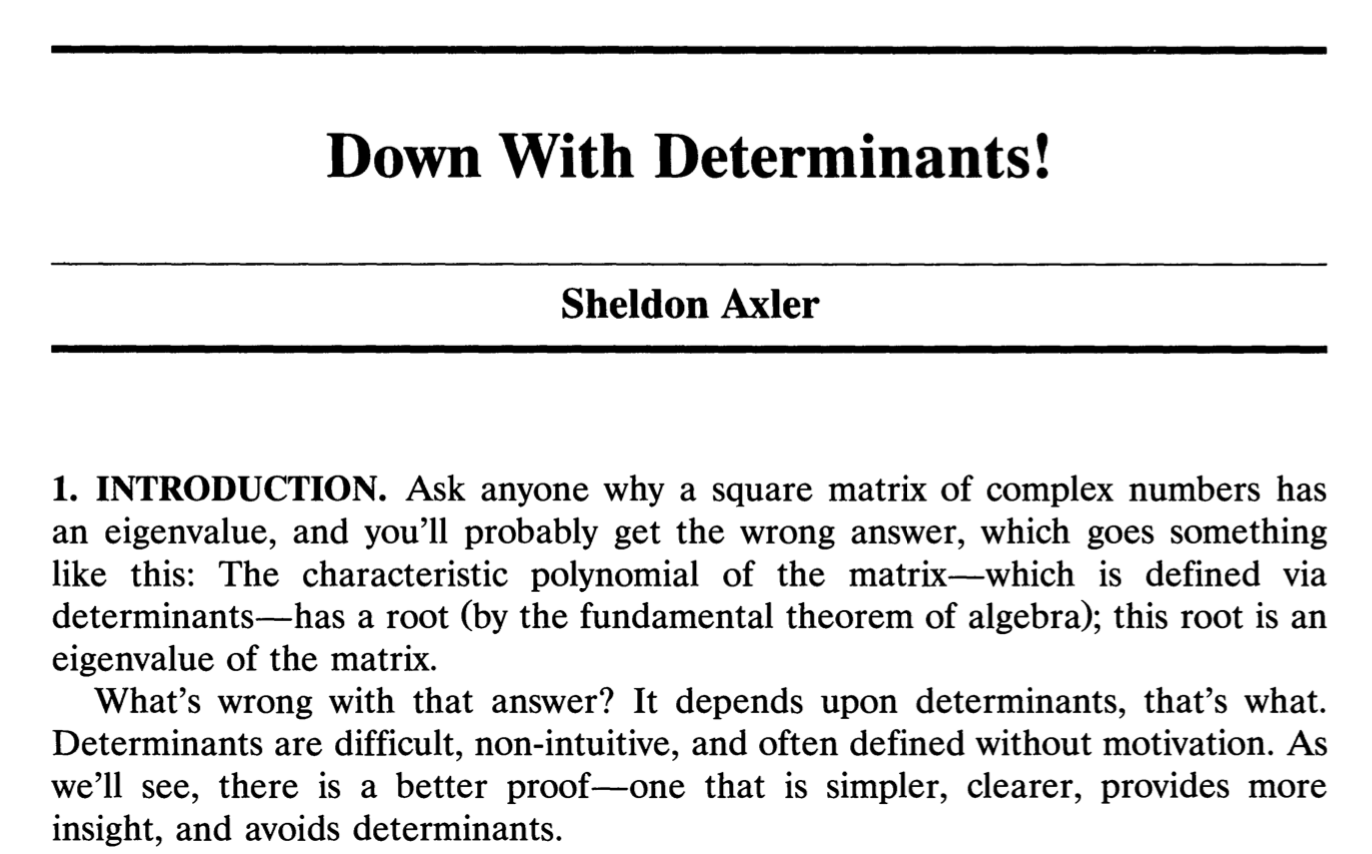
\includegraphics[width=.72\textwidth]{figs/down-with-determinants.png}
  \end{frame}

  \begin{frame}
    \frametitle{And yet... Determinantal Point Processes (DPPs)}
A family of \underline{non-i.i.d.}~sampling distributions\pause
    
    \begin{enumerate}
    \item Applications in Randomized Linear Algebra\pause
      \begin{itemize}
      \item Least squares regression \cite{unbiased-estimates,leveraged-volume-sampling}\pause
      \item Low-rank approximation
        \cite{pca-volume-sampling,more-efficient-volume-sampling,nystrom-multiple-descent}\pause
        \item Randomized Newton's method \cite{determinantal-averaging,randomized-newton}
        \end{itemize}\pause
      \item Connections to i.i.d.~sampling methods\pause
        \begin{itemize}
        \item Row norm scores\pause
        \item Leverage scores\pause
        \item Ridge leverage scores\pause
        \end{itemize}
      \item Fast DPP sampling algorithms\pause
        \begin{itemize}
        \item Exact sampling via eigendecomposition \cite{dpp-independence,k-dpp}\pause
        \item Intermediate sampling via leverage scores
          \cite{dpp-intermediate,dpp-sublinear}\pause
        \item Markov chain Monte Carlo sampling \cite{rayleigh-mcmc}
        \end{itemize}
    \end{enumerate}
  \end{frame}

\section{Determinantal point processes}
  
  \begin{frame}
    \frametitle{L-ensemble DPPs and k-DPPs}
  Given a psd $n\times n$ matrix $\L$, sample subset
  $S\subseteq\{1..n\}$:
  \begin{align*}
\text{(L-ensemble)}\quad\DPP(\L):&\quad    \Pr(S) =
                                   \frac{\det(\L_{S,S})}{\Blue{\det(\I+\L)}}\quad
                                   \text{over all subsets}.\\
\onslide<2->{&\qquad\qquad\quad\text{\Blue{closed form normalization!}}}\\
\onslide<3->{\text{(k-DPP)}\quad k\text{-}\DPP(\L):&\quad \DPP(\L)\text{ conditioned on }|S|=k.}
  \end{align*}  
  \pause\pause\pause
  DPPs appear everywhere!\pause
  \begin{itemize}
  \item Physics \hfill \small (fermions)\pause
  \item Random matrix theory \hfill \small (eigenvalue distribution)\pause
  \item Graph theory \hfill \small (random spanning trees)\pause
  \item Optimization \hfill \small (variance reduction)\pause
  \item Machine learning \hfill \small (diverse sets)
  \end{itemize}
\end{frame}

\begin{frame}
  \frametitle{Volume (determinant) as a measure of diversity}
  Let $\L=\big[\x_i^\top\x_j\big]_{ij}$ for
  $\x_1,\dots,\x_n\in\R^d$. \\
\pause  Then, $\det(\L_{S,S}) =
\mathrm{Vol}^2\big(\{\x_i:i\in S\}\big)$
\pause

  \centering
  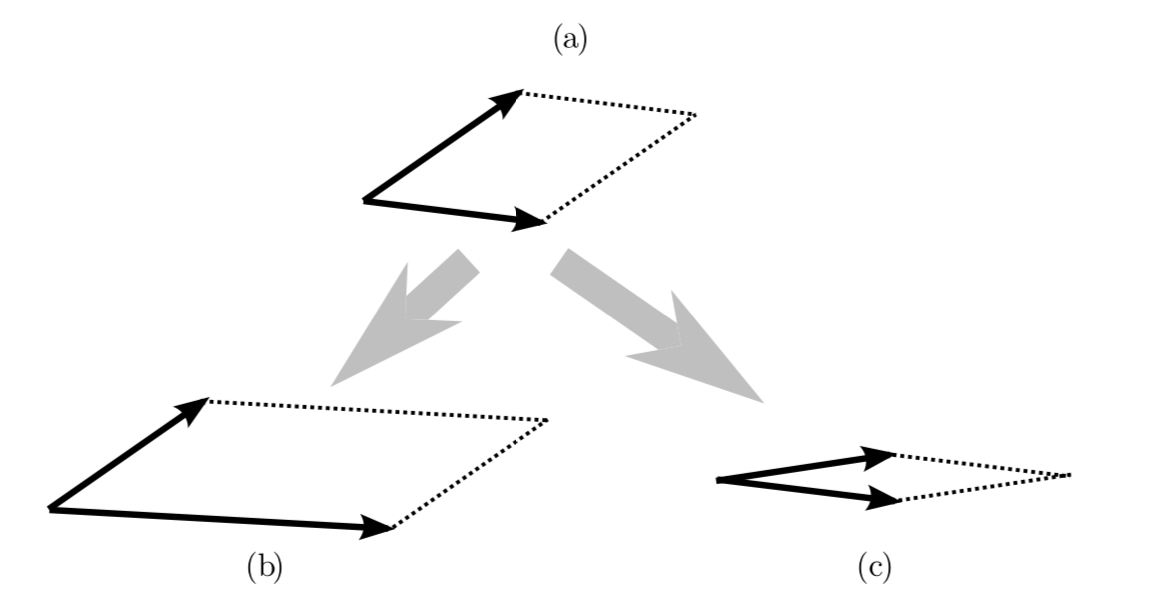
\includegraphics[width=\textwidth]{../figs/volume_illustration.png}
    \let\thefootnote\relax\footnotetext{Image from \cite{dpp-ml}}
\end{frame}

\begin{frame}
  \frametitle{Example: DPP vs i.i.d.}
  \underline{Negative correlation}:
  $\Pr(i\in S\mid j\in S) < \Pr(i\in S)$
  \pause
\begin{center}
  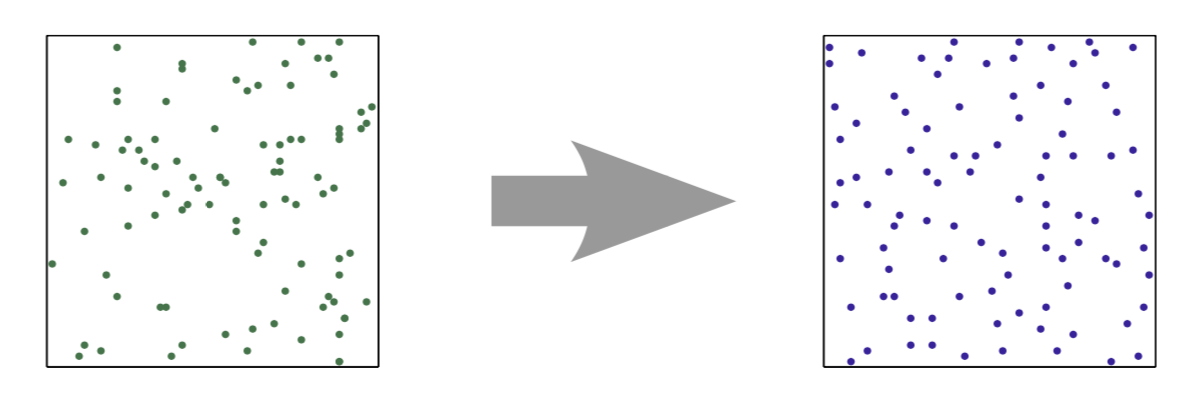
\includegraphics[width=0.8\textwidth]{../figs/gue.png}
  
  \small  i.i.d.~(left) versus DPP (right)%
  \end{center}
    \let\thefootnote\relax\footnotetext{Image from \cite{dpp-ml}}
\end{frame}


\begin{frame}
  \frametitle{Projection DPPs}
  If $\L$ has rank $d$, then $S\sim d$-$\DPP(\L)$ is a
  \underline{Projection DPP}\\[10mm]\pause
Let $\L=\X\X^\top$ for a full rank $n\times d$ matrix $\X$\vspace{-2mm}
\begin{align*}
\text{if}\quad S\sim d\text{-}\DPP(\L)\quad\text{then}\quad\Pr(S) = \frac{\det(\X_S)^2}{\Blue{\det(\X^\top\X)}}.
\end{align*}
\vspace{-4mm}
\pause

\Blue{Closed form normalization (Cauchy-Binet formula).}
\pause
\vspace{10mm}

\textbf{Remark}. If $k<\rank(\L)$ then $k$-$\DPP(\L)$ is \emph{not} a
projection DPP.\\
(and also does not have such a simple normalization constant)
\end{frame}

\begin{frame}
  \frametitle{Hierarchy of DPPs}
  Broader class of negatively-correlated point processes:\\
  \textit{Strongly Rayleigh (SR) measures}
  \vspace{5mm}
  
\begin{center}
  \begin{tikzpicture}[scale=1.1]
    \draw [fill=purple!10,opacity=.5] (3.25,2.2) ellipse (4 and 2);
    \draw (3.25,3.95) node {SR measures};                              
    \draw [fill=blue!70,opacity=.5] (2,2) ellipse (2 and 1.5);
    \draw (2,3.3) node {DPPs};
    \draw [fill=blue!10,opacity=.5] (2,2) ellipse (1.47 and 1.05);
    \draw (2,2.5) node {L-ensembles};                        
    \draw [fill=red!50,opacity=.5] (5,2) ellipse (1.47 and 1.05);
    \draw (5,2.5) node {k-DPPs};
    \draw [thick,<-] (3.8,2) -- (3.9,3.15);
    \draw (4.75,3.3) node {{\small Projection DPPs}};
  \end{tikzpicture}
  \end{center}
\end{frame}

\begin{frame}
  \frametitle{Random vs fixed subset size}
Let $d=\rank(\L)$, and $\lambda_1,...,\lambda_d$ be the non-zero
eigenvalues of $\L$\\
If $S\sim\DPP(\L)$ then:
  \begin{align*}
\quad   |S|&\sim
    \text{Poisson-Binomial}\big(\tfrac{\lambda_1}{\lambda_1+1},...,\tfrac{\lambda_d}{\lambda_d+1}\big)\\
    \onslide<2->{    \E\big[|S|\big]
       &= \sum_{i=1}^d\frac{\lambda_i}{\lambda_i+1}
= \tr\big(\L(\L+\I)^{-1}\big)<d}
  \end{align*}
  \pause
  \pause
  \underline{Rescaling trick:} \ Sample $S\sim \DPP(\frac1\lambda\L)$ to
  control $\E[|S|]$
  \pause
  \begin{align*}
\Pr(S)\propto    \det(\tfrac1\lambda\L_{S,S}) = \lambda^{-|S|}\det(\L_{S,S})
  \end{align*}\pause
  \begin{align*}
    \underbrace{\DPP\big(\tfrac1{\lambda}\L\big)}_{\text{L-ensemble}}
    \ \ \overset{\lambda\rightarrow 0}\longrightarrow\
    \underbrace{d\text{-}\DPP\big(\L\big)}_{\text{Projection DPP}}
  \end{align*}
\end{frame}

\section{DPPs in Randomized Linear Algebra}

\begin{frame}
  \frametitle{DPPs in Randomized Linear Algebra}
  \underline{Given}: data matrix $\X$ \\[2mm]
\underline{Goal} (row sampling): construct $\Xt$ from few
rows  of $\X$\vspace{2mm}
  \begin{center}
\hspace{2cm}  \begin{tikzpicture}[scale=0.5]
  \draw (0,0) rectangle (2,4);
  \draw[fill=blue!20] (0,1.5) rectangle (2,3.5);
    \draw (-.4,3.5) node {\mbox{\footnotesize $\X$}};  
    \draw (1,2.75) node {\mbox{\footnotesize $\Xt$}};
    \draw (.7,-.7) node {\textit{Rank-preserving sketch}};
  \end{tikzpicture}
  \begin{tikzpicture}[scale=0.5]
    \draw (0,0) rectangle (4,4);
    \draw[fill=blue!20] (0,1.8) rectangle (4,3.5);
    \draw (-.4,3.5) node {\mbox{\footnotesize $\X$}};  
    \draw (2,2.75) node {\mbox{\footnotesize $\Xt$}};
    \draw (1.8,-.7) node {\textit{Low-rank approximation}};
  \end{tikzpicture}
\end{center}

\underline{i.i.d.~sampling}:\only<2->{\hspace{6mm} \textit{Leverage
  scores}\hspace{1cm} \textit{Ridge leverage scores}}
\vspace{3mm}

\underline{DPP sampling}:\only<3->{\hspace{4mm} \textit{Projection
    DPPs}\hspace{1.7cm} \textit{L-ensembles}}
\end{frame}

\begin{frame}
  \frametitle{Connections to i.i.d.~sampling}
  \underline{Given}: full rank $n\times d$ matrix $\X$\\[2mm]
Methods based on i.i.d.~row sampling:\pause
  \begin{enumerate}
    \item Row norm scores:
      $p_i=\frac{\|\x_i\|^2}{\|\X\|_F^2}$\pause\vspace{-3mm}
      \begin{align*}
        \tfrac{\|\x_i\|^2}{\|\X\|_F^2} = \Pr\big(i\in S\big)
        \quad\text{ for }\quad
        S\sim 1\text{-}\DPP(\X\X^\top)
      \end{align*}\pause\vspace{-5mm}
    \item Leverage scores: $p_i=\frac1d\x_i^\top(\X^\top\X)^{-1}\x_i$\pause\vspace{-3mm}
      \begin{align*}
        \x_i^\top(\X^\top\X)^{-1}\x_i = \Pr\big(i\in S\big)\quad\text{ for }\quad
        S\sim d\text{-}\DPP(\X\X^\top)
      \end{align*}\pause\vspace{-5mm}
    \item Ridge leverage scores: $p_i =\frac1{d_\lambda}
      \x_i^\top(\X^\top\X+\lambda\I)^{-1}\x_i$\pause\vspace{-3mm}
      \begin{align*}
        \x_i^\top(\X^\top\X+\lambda\I)^{-1}\x_i &= \Pr\big(i\in S\big)\quad\text{ for }\quad
        S\sim \DPP(\tfrac1\lambda\X\X^\top)
      \end{align*}
    \end{enumerate}      
  \end{frame}

  \begin{frame}
    \frametitle{Subsampled least squares}
{\bf Given}: $n$ points $\x_i\in\R^d$ with labels $y_i\in \R$\\
{\bf Goal}: Minimize loss $L(\w)= \sum_i (\x_i^\top\w-y_i)^2$ over
all $n$ points
\begin{align*}
\w^*=\argmin_\w L(\w) = \X^\dagger\y
\end{align*}
\only<1>
{
\begin{columns}
\begin{column}{0.3\textwidth}
\end{column}
\begin{column}{0.5\textwidth}
\begin{center}
	\begin{tikzpicture}[scale=0.9]
          \draw [fill=brown!30] (-2,0) rectangle (0,3);
          \draw [decorate,decoration={brace}] (-2.1,0) -- (-2.1,3);
          \draw (-2.4,1.51) node {\mbox{\fontsize{8}{8}\selectfont $n$}}; 
          \draw [decorate,decoration={brace}] (-2,3.1) -- (0,3.1);
          \draw (-1,3.4) node {\mbox{\fontsize{8}{8}\selectfont $d$}}; 

	    \draw (-2.5,3) node {$\X$}; 
            \draw [color=grey,line width =0.5mm] (1,0) -- (1,3);
            \draw [] (0.75,3) node {$\y$};
	\end{tikzpicture}
\end{center}
\end{column}
\end{columns}
}
\only<2->
{
\begin{columns}
\begin{column}{0.32\textwidth}
\\\vspace{0.65cm}
Sample $S=\{4,6,9\}$\\
\vspace{1cm}
Solve subproblem $(\X_S,\y_S)$
\end{column}
\begin{column}{0.5\textwidth}
\begin{center}
	\begin{tikzpicture}[scale=0.9]
          \draw [fill=brown!30] (-2,0) rectangle (0,3);
          \draw [color=black] (-2,2) -- (0,2);
          \draw (-2.25,2) node {\mbox{\footnotesize $\x_4^\top$}}; 
          \draw [color=black] (-2,1.5) -- (0,1.5);
          \draw (-2.25,1.5) node {\mbox{\footnotesize $\x_6^\top$}}; 
          \draw [color=black] (-2,0.5) -- (0,0.5);
          \draw (-2.25,0.5) node {\mbox{\footnotesize $\x_9^\top$}}; 
	   \draw (-2.5,3) node {$\X$}; 
           \draw [decorate,decoration={brace}] (-2,3.1) -- (0,3.1);
          \draw (-1,3.4) node {\mbox{\fontsize{8}{8}\selectfont $d$}}; 
            \draw [color=gray,line width =0.5mm] (1,0) -- (1,3);
            \draw [] (0.75,3) node {$\y$};
            \draw (0.75,2) node {\mbox{\footnotesize $y_4$}}; 
            \draw (1,2) node {.}; 
            \draw[mark=*,mark size=1.5pt] plot coordinates{(1,2)};
            \draw (0.75,1.5) node {\mbox{\footnotesize $y_6$}}; 
            \draw (1,1.5) node {.}; 
            \draw[mark=*,mark size=1.5pt] plot coordinates{(1,1.5)};
            \draw (0.75,0.5) node {\mbox{\footnotesize $y_9$}}; 
            \draw[mark=*,mark size=1.5pt] plot coordinates{(1,.5)};
	\end{tikzpicture}
\end{center}
\end{column}
\end{columns}
}
\end{frame}

\begin{frame}
  \frametitle{Unbiased estimators}
  \begin{theorem}[Rank-preserving sketch, \cite{unbiased-estimates}]
    If $S\sim d$-$\DPP(\X\X^\top)$, then:\vspace{-3mm}
    \begin{align*}
      \E[\X_S^{-1}\y_S] =
      \overbrace{\argmin_{\w}L(\w)=\w^*}^{\text{least squares}}.
      \end{align*}
    \end{theorem}
    \pause

    \begin{theorem}[Low-rank sketch, \cite{surrogate-design}]
      If $S\sim \DPP(\frac1\lambda\X\X^\top)$, then: \vspace{-3mm}
      \begin{align*}
\E[\X_S^\dagger\y_S]=\overbrace{\argmin_\w L(\w)+
        \lambda\|\w\|^2}^{\text{ridge regression}}
        \end{align*}
      \end{theorem}
      \pause
      Not achievable with any i.i.d.~row sampling!
\end{frame}

\begin{frame}
  \frametitle{Merits of unbiased estimators}
Simple Strategy: \\
1. Compute independent estimators $\w(S_j)$ for $j=1,..,k$,\\
2. Predict with the average estimator $\frac{1}{k}\sum_{j=1}^k\w(S_j)$\\[4mm]
\pause
If we have 
\begin{align*}
\E[L(\w(S))]\leq (1+c)L(\w^*)
\quad\text{and}\quad\E[\w(S)]=\w^*,
\end{align*}
then for $k$ independent samples $S_1,\ldots,S_k$,
$$\E\bigg[L\Big(\frac{1}{k}\sum_{j=1}^k \w(S_j) \Big)\bigg]
  \leq \left(1 + \frac{c}{k}\right)L(\w^*)$$
%Thus we need $s\underbrace{c/\epsilon}_k$ responses to get a $(1+\epsilon)$ approximation
\pause
Motivation:
\begin{itemize}
\item Ensemble methods
\item Distributed optimization
\item Privacy
\end{itemize}
\end{frame}

\begin{frame}
  \frametitle{Connections to Gaussian sketches}
  \underline{Gaussian sketch}\\
  (Also gives \textit{unbiased} estimators for least squares)\\[2mm] \pause
  Let $\S$ be $\frac1{k}\times$\,i.i.d.~Gaussian with $\E[\S^\top\S]=\I$. For $k>d+1$:
  \begin{align*}
\E\big[(\X^\top\S^\top\S\X)^{-1}\big] = (\X^\top\X)^{-1}\frac{k}{k-d-1}
  \end{align*}
  \pause\vspace{3mm}

  \underline{DPP plus uniform}\\
  Let $S\sim d$-$\DPP(\X\X^\top)$, 
  $T\sim\mathrm{Bin}(n,\frac{k-d}{n-d})$ and
$\bar\S = \big[\sqrt{\!\frac nk}\,\e_i\big]_{i\in S\cup
  T}^\top$. \\
Note: $\E[|S|]=k$. For $k\geq d$, we have:
  \begin{align*}
    \E\big[(\X^\top\bar\S^\top\bar\S\X)^{-1}\big] =
    (\X^\top\X)^{-1}\frac{k}{k-d}\cdot \big(1-o_n(1)\big)
  \end{align*}
  \pause
  \begin{block}{}
    DPPs have a ``Gaussianizing'' effect on row sampling.
  \end{block}
\end{frame}

\section{Key technique: \textit{Determinant preserving random matrices}}

\begin{frame}
  \frametitle{Determinant preserving random matrices}
\begin{definition}[\cite{surrogate-design}]
A random $d\times d$ matrix $\A$ is \emph{determinant preserving} (d.p.) if
\begin{align*}
  \E\big[\!\det(\A_{\Ic,\Jc})\big] =
  \det\!\big(\E[\A_{\Ic,\Jc}]\big)\quad \text{for all }\Ic,\Jc\subseteq
  [d]\text{ s.t. }|\Ic|=|\Jc|.
\end{align*}
\vspace{-7mm}
\end{definition}
\vspace{5mm}

Basic examples: \pause
\begin{itemize}
\item Every \textit{deterministic} matrix \pause
\item Every \textit{scalar} random variable \pause
\item Random matrix with i.i.d.~Gaussian entries
\end{itemize}
\end{frame}

\begin{frame}
  \frametitle{More examples}
  Let $\A = s\,\Z$, where:
  \begin{itemize}
  \item $\Z$ is deterministic with $\rank(\Z) = r$,
  \item $s$ is a scalar random variable with positive variance.
  \end{itemize}\vspace{1mm}
\pause
  \begin{align*}
  \E\big[\det(s\,\Z_{\Ic,\Jc})\big] &= \E[s^r]\det(\Z_{\Ic,\Jc})
=\det\Big(\big(\E[s^r]\big)^{\frac1r}\,\Z_{\Ic,\Jc}\Big),
  \end{align*}
  \pause
  
Two cases:
\begin{enumerate}
\item If $r=1$ then $\A$ is determinant preserving,
  \item If $r>1$ then $\A$ is \underline{not}
    determinant preserving.
    \end{enumerate}
\end{frame}

\begin{frame}
  \frametitle{Basic properties}
  \begin{lemma}[Closure]
  If $\A$ and $\B$ are independent and determinant preserving, then:
  \begin{itemize}
  \item $\A+\B$ is determinant preserving,
  \item $\A\B$ is determinant preserving.
    \end{itemize}
  \end{lemma}
  \pause\vspace{5mm}
  
  \begin{lemma}[Adjugate]
    If $\A$ is determinant preserving, then  $\E[\adj(\A)]=\adj(\E[\A])$.
  \end{lemma}
When $\A$ is invertible then $\adj(\A) = \det(\A)\A^{-1}$\vspace{5mm}

\footnotesize{Note: The $(i,j)$th entry of $\adj(\A)$ is
$(-1)^{i+j}\det(\A_{[n]\backslash\{j\},[n]\backslash\{i\}})$.}
\end{frame}

\begin{frame}
  \frametitle{Proof of closure under addition}
First show that $\A+\u\v^\top$ is d.p.~for fixed $\u,\v\in\R^d$:\pause
  \begin{align*}
\E\big[\!\det(\A_{\Ic,\Jc}\!+\u_{\Ic}\v_{\Jc}^\top)\big] &=
    \E\big[\!\det(\A_{\Ic,\Jc}) +
    \v_{\Jc}^\top\adj(\A_{\Ic,\Jc}) \u_{\Ic}\big]\\
\onslide<3->{    &=\det\!\big(\E[\A_{\Ic,\Jc}]\big) +
      \v_{\Jc}^\top\adj\!\big(\E[\A_{\Ic,\Jc}]\big) \u_{\Ic}}\\
\onslide<4->{    &=\det\!\big(\E[\A_{\Ic,\Jc} \!+ \u_{\Ic}\v_{\Jc}^\top]\big).}
  \end{align*}
  \pause\pause\pause
  Iterating this, we get $\A+\Z$ is d.p.~for any fixed $\Z$\\
  \pause
    \begin{align*}
\E\big[\!\det(\A_{\Ic,\Jc}\!+\B_{\Ic,\Jc})\big]
    &=
      \E\Big[\E\big[\!\det(\A_{\Ic,\Jc}\!+\B_{\Ic,\Jc})\mid\B\big]\Big]\\
   \onslide<7->{ &=\E\Big[\!\det\!\big(\E[\A_{\Ic,\Jc}]\!+\B_{\Ic,\Jc}\big)\Big]}\\
\onslide<8->{ &= \det\!\big(\E[\A_{\Ic,\Jc}\!+\B_{\Ic,\Jc}]\big)}
  \end{align*}
\pause\pause\hfill\qed

\end{frame}

\begin{frame}
  \frametitle{Application: Expected inverse}
  \begin{theorem}
Let  $\Pr(S) \propto
\det(\X_S^\top\X_S)p^{|S|}(1-p)^{n-|S|}$ over all $S\subseteq[n]$. Then:
    \begin{align*}
    \E\big[(\X_S^\top\X_S)^{-1}\big] \preceq \tfrac1p\,(\X^\top\X)^{-1}.
  \end{align*}
\end{theorem}
\pause
\textbf{Proof} \
Let $b_1,...,b_n\sim\mathrm{Bernoulli}(p)$, and define $\bar S=\{i:b_i=1\}$\\\pause
For each $i\in[n]$, matrix $b_i\x_i\x_i^\top$ is determinant preserving \\\pause
Therefore, $\X_{\bar S}^\top\X_{\bar S}=\sum_{i=1}^nb_i\x_i\x_i^\top$
is determinant preserving\pause
\begin{align*}
  \E\big[(\X_S^\top\X_S)^{-1}\big]
  &=
    \frac{\E[\det(\X_{\bar S}^\top\X_{\bar S})(\X_{\bar
    S}^\top\X_{\bar S})^\dagger]}{\E[\det(\X_{\bar S}^\top\X_{\bar S})]}
   \only<6->{ \preceq \frac{\E[\adj(\X_{\bar S}^\top\X_{\bar
    S})]}{\E[\det(\X_{\bar S}^\top\X_{\bar S})]}}\\
\onslide<7->{  &=\frac{\adj(\E[\X_{\bar S}^\top\X_{\bar S}])}{\det(\E[\X_{\bar
    S}^\top\X_{\bar S}])}}\onslide<8->{ = \big(\E[\X_{\bar S}^\top\X_{\bar S}]\big)^{-1}}\onslide<9->{\!\!=(p\X^\top\X)^{-1}}
\end{align*}
\pause\pause\pause\pause\hfill\qed
\end{frame}

\section{Sampling algorithms}

\begin{frame}
  \frametitle{Algorithmic challenges with sampling from DPPs}
  \textbf{Task:}
  \begin{quote}
(variant 1)\quad Given $\L$, sample $S\sim\DPP(\L)$\\
(variant 2)\quad Given $\L$ and $k$, sample $S\sim
  k\text{-}\DPP(\L)$
  \end{quote}
\pause 
(Task B:\quad we are given $n\times d$ matrix $\X\in\R^d$ instead of $\L=\X\X^\top$) 
\pause  \vspace{4mm}

  \textbf{Challenges:}
  \begin{enumerate}
  \item Expensive preprocessing \\[-1mm]
{\small typically involves eigendecomposition
  of $\L$ in $O(n^3)$ time}\pause
\vspace{2mm}
\item Sampling time scales with $n$ rather than with $|S|\ll n$\\[-1mm]
{\small undesirable when we need many samples
  $S_1,S_2,\dots\sim\DPP(\L)$}\pause
\vspace{2mm}
\item Trade-offs between accuracy and runtime\\[-1mm]
  {\small   \begin{itemize}
\item \underline{exact} algorithms -  often too expensive
\item  \underline{approximate} algorithms - difficult to evaluate accuracy
\end{itemize} }
\end{enumerate}
\end{frame}

\begin{frame}
  \frametitle{Exact DPP sampling}
  \textbf{Key result:} any DPP is a \underline{mixture of Projection
    DPPs} \cite{dpp-independence}\pause
  \vspace{1mm}
  \begin{itemize}
  \item  Eigendecomposition\quad $O(n^3)$\\[-2mm]
{\footnotesize needed only once for a given kernel}
\item Reduction to a projection DPP\quad $O(n\,|S|^2)$\\[-2mm]
  {\footnotesize needed for every sample}
    \end{itemize}
    \pause
    \vspace{5mm}
    
    \begin{block}{}
  \begin{itemize}
  \item Cost of first sample $S_1\sim\DPP(\L)$:\quad $O(n^3)$\pause
    \item Cost of next sample $S_2\sim\DPP(\L)$:\quad$O(nk^2)$\hfill$(k=\E[|S|])$
    \end{itemize}
    \end{block}\pause
    Extends to a k-DPP sampler \small\cite{k-dpp}
    
\end{frame}

\begin{frame}
  \frametitle{Approximate k-DPP sampler using MCMC}
  \begin{enumerate}
  \item Start from some state $S\subseteq[n]$ of size $k$\pause
  \item Uniformly sample $i\in S$ and $j\not\in S$\pause
  \item Move to state $S-i+j$ with probability $\frac12
    \min\Big\{1,\frac{\det(\L_{S-i+j})}{\det(\L_S)}\Big\}$\pause
    \item ...
    \end{enumerate}
    Converges in $O(nk\log\frac1\epsilon)$ steps to within $\epsilon$
    total variation \cite{rayleigh-mcmc}
    \pause\vspace{2mm}
    \begin{block}{}
  \begin{itemize}
  \item Cost of first sample $S_1\sim k\text{-}\DPP(\L)$:\quad $O(n\cdot\poly(k))$\pause
    \item Cost of next sample $S_2\sim k\text{-}\DPP(\L)$:\quad$O(n\cdot\poly(k))$
    \end{itemize}
  \end{block}\pause
Extends to an $O(n^2\cdot\poly(k))$ sampler for $\DPP(\L)$ \ \small\cite{kdpp-mcmc}
  
\end{frame}

\begin{frame}
  \frametitle{Distortion-free intermediate sampling}  
  \begin{columns}
    \begin{column}{0.55\textwidth}
  \begin{enumerate}
  \item[\Blue{1.}] Draw an intermediate sample:\\[-1mm]
    ~\hfill $\sigma=(\sigma_1,\dots,\sigma_t)$
  \item[\Red{2.}] Downsample: \ \,$S\subseteq[t]$
\item[3.] Return: \qquad\ \ $\{\sigma_i:i\in S\}$
  \end{enumerate}
\end{column}
\begin{column}{0.45\textwidth}
  \begin{center}
\begin{tikzpicture}
    \path 
        (0,0) rectangle (5,3) [draw]
        (0.6,2.6) node {$\{1..n\}$}
        (2.4,1.4) coordinate (A) node[left]
        {$\overset{\Red{(2)}}{S}$\hspace{-1mm}~} ellipse (2.3 and 1.2) [draw] 
        coordinate (temp) at (2.5,2)    ellipse (0.6 and 0.6) [draw]
        (temp) +(1,0.1) coordinate (B) node[left]
        {$\overset{\Blue{(1)}}{\sigma}$}; % --
\end{tikzpicture}
\end{center}
\end{column}
\end{columns}
\pause
\vspace{10mm}

What is the right intermediate sampling distribution for $\sigma$?\pause
\begin{itemize}
  \item \underline{Leverage scores}, when $S$ is a Projection DPP\pause
  \item \underline{Ridge leverage scores}, when $S$ is an L-ensemble
\end{itemize}
\end{frame}


\begin{frame}
  \frametitle{Distortion-free intermediate sampling for L-ensembles} 
  \begin{theorem}[\cite{dpp-sublinear}]
There is an algorithm which, given access to $\L$, returns
\begin{enumerate}
\item first sample $S_1\sim\DPP(\L)$ in:\quad $n\cdot\poly(k)\,\polylog(n)$ time,
\item next sample $S_2\sim\DPP(\L)$ in:\hspace{6.4mm}  $\poly(k)$ time.
  \end{enumerate}
\end{theorem}
\pause

\begin{itemize}
\item Exact sampling\pause
\item Cost of first sample is \emph{sublinear} in the size of $\L$\pause
\item Cost of next sample is \emph{independent} of the size of $\L$
\end{itemize}
\end{frame}

\section{Conclusions}

\begin{frame}
  \frametitle{Conclusions}

  \begin{enumerate}
  \item New fundamental connections between:
    \begin{enumerate}
      \item Determinantal Point Processes
      \item Randomized Linear Algebra
      \end{enumerate}\pause\vspace{2mm}
    \item New unbiased estimators and expectation
      formulas\vspace{2mm}\pause
      \item Efficient sampling algorithms\vspace{2mm}\pause
    \item \textit{Determinant preserving random matrices}
    \end{enumerate}
    \pause
    \vspace{5mm}
    {\footnotesize
DPP-related topics we did not cover:\vspace{-2mm}
    \begin{itemize}
    \item Column Subset Selection Problem\vspace{-3mm}
    \item Nystr\"om method\vspace{-3mm}
    \item Monte Carlo integration\vspace{-3mm}
    \item Distributed/Stochastic optimization\vspace{-3mm}
    \item ...
    \end{itemize}}
\end{frame}

\begin{frame}[allowframebreaks]
  \frametitle{References}
  \tiny
  \bibliographystyle{alpha}
  \bibliography{../pap}
\end{frame}

\begin{frame}
\centering  \Large Thank you!
\end{frame}


\end{document}